% Chapter Template

\chapter{Introduction} % Main chapter title

\label{Chapter1} % Change X to a consecutive number; for referencing this chapter elsewhere, use \ref{ChapterX}

%----------------------------------------------------------------------------------------
%	SECTION 1
%----------------------------------------------------------------------------------------

\section{Why we need numerical relativity?}

General relativity is the theory that best describes modern cosmology, celestial bodies such as black holes, and gravitational waves. In general relativity, Einstein's field equation describes curved spacetime as the momentum and energy of matter.

However, these are ten nonlinear partial differential equations, whose complete solutions have not yet been solved analytically, except for the Friedmann–Lemaître–Robertson–Walker metric, etc. With advances in computer algorithms and physics, Einstein's equations began to be solved numerically, which is the beginning of numerical relativity.

\section{Introduction to numerical relativity}
In numerical relativity, Einstein's equations is separated into space part and time part, that is, 3+1 decomposition.

\begin{figure}[H]
	\centering
	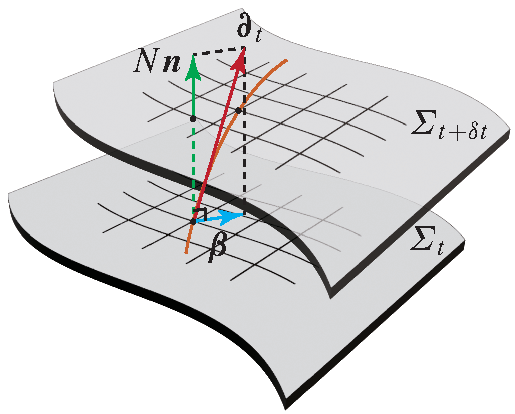
\includegraphics{Figures/foliation.pdf}
	\caption{A foliation of the spacetime. There are time vector $\timevec$, normal evolution vector $N\bm{n}$, and shift vector $\shiftvec$ satisfying $\timevec = N\bm{n} + \shiftvec$ between the two hypersurfaces $\Sigma_t$, $\Sigma_{t+\delta t}$.}
	\label{fig:foliation}
\end{figure}

From this, it is possible to calculate the next spatial metric from the initial condition of the space at a specific time. This is done in a similar way as in Newtonian classical mechanics, given the initial position and velocity of an object, the position and velocity at the next time can be calculated using the acceleration due to the force acting on the object. However, unlike in Newtonian mechanics, the initial value must satisfy certain specific conditions. Therefore, the calculation is made by first constructing the initial data, selecting the appropriate coordinates, and then evolving it from the numerical method.

\begin{figure}[H]
	\centering
	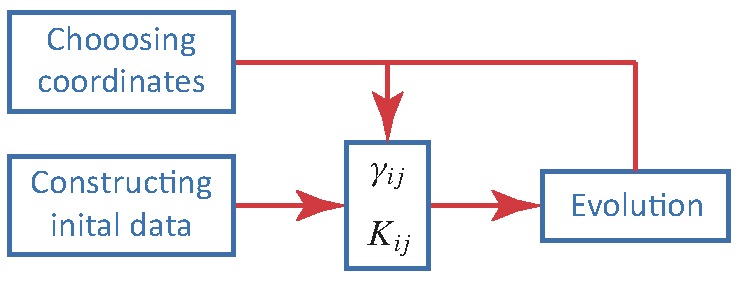
\includegraphics{Figures/scheme.pdf}
	\caption{A brief schema of numerical relativity.}
	\label{fig:scheme}
\end{figure}

In this work, we try to numerically evolve the Schwarzschild metric from its initial conditions to understand the basic way of working with numerical relativity.

\section{Notation and conventions}
%\subsection{Sign conventions}
Throughout this report, we follows the ``Landau-Lifshitz Spacelike Convention''($- + + +$) as \parencite{misner1973gravitation}. Also we will adopt a units for measurements in which both the gravitational constant $G$ and the speed of light $c$ are assigned the values of one.

We denote the dimension 4 spacetime metric by $g_{ab}$, the dimension 3 spatial metric
by $\gamma_{ij}$. Also the dimension 4 objects associated with $g_{ab}$ are denoted with a superscript ${}^{(4)}$ in front of the symbol, objects related to $\gamma_{ij}$ carry no decorations.